%
%  untitled
%
%  Created by Johan Boissard [] on 2010-06-24.
%  Copyright (c) Johan Boissard. All rights reserved.
% hhh

\documentclass[a4paper] {scrartcl}
\usepackage[T1]{fontenc}
\usepackage[utf8]{inputenc}
\usepackage{graphicx}
\usepackage{engord}
%\usepackage[english]{babel}
\usepackage{fancyhdr}
\usepackage{amsmath}
\usepackage{comment}

\usepackage{listings}

%allows inclusion of url (hyperref is better than url) 
%ref: http://www.fauskes.net/nb/latextips/
\usepackage{hyperref}

%package for chemistry ie: \ce{(NH4)2SO4 -> NH4+ + 2SO4^2-} 
%ref:www.ctan.org/tex-archive/macros/latex/contrib/mhchem/mhchem.pdf
\usepackage[version=3]{mhchem}
%celsius + degrees
\usepackage{gensymb}
%to get last page
\usepackage{lastpage} % \pageref{LastPage}

%make use of the fullpage (no HUGE margins)
\usepackage{fullpage}
\usepackage{subfig}

%allows separating cell in table by diagonal line
\usepackage{slashbox}




%\renewcommand{\chaptername}{Laboratory}
%\setcounter{chapter}{5}

\usepackage{color}
\usepackage[usenames,dvipsnames, table]{xcolor}
% Include this somewhere in your document



\usepackage[absolute]{textpos}

%column  of multi row in tables
\usepackage{multirow}

%to have vertical text in table
\usepackage{rotating}


%%%%%%% a virer ici!!!!
\begin{comment}
%Fonts and Tweaks for XeLaTeX
\usepackage{fontspec,xltxtra,xunicode}
%\defaultfontfeatures{Mapping=tex-text}
%\setromanfont[Mapping=tex-text]{Hoefler Text}
\setsansfont[Scale=MatchLowercase,Mapping=tex-text]{Gill Sans}

\definecolor{shade}{HTML}{D4D7FE}	%light blue shade
\definecolor{text1}{HTML}{272727}		%text is almost black
\definecolor{headings}{HTML}{173849} 	%dark blue %%%dark red 70111
\definecolor{title}{HTML}{173849} 	%dark blue %%%dark red 70111

\usepackage{titlesec}				%custom \section
\end{comment}







\author{Johan Boissard}
\date{\today}
\title{MacroEconomics}
\begin {document}

\maketitle
%\tableofcontents


\section{Macroeconomics Essentials} % (fold)
\label{sec:macroeconomics_essentials}


\subsection{Issues of macroeconomics} % (fold)
\label{sub:issues_of_macroeconomics}



\begin{itemize}
	\item GDP: gross domestic product: measures total income (or output). income generated within geogrpahical boundaries
	\item GNP $\equiv$ GNI (gross national income): gross national product (separated) : income generated by inhabitants of country
\end{itemize}


% subsection issues_of_macroeconomics (end)


\subsection{Macroeconomics Essentials} % (fold)
\label{sub:macroeconomics_essentials}


\begin{figure}[htbp]
	\centering
		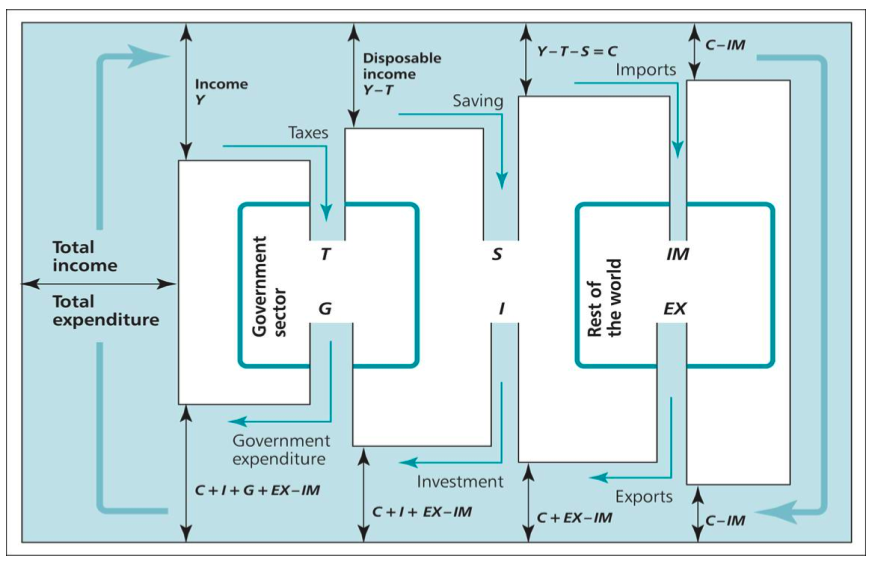
\includegraphics[height=3in]{images/circularflow.png}
	\caption{Circular Flow}
	\label{fig:images_circularflow}
\end{figure}

\begin{equation}
	(S-I) + (T-G) + (IM-EX) = 0
\end{equation}
where
\begin{itemize}
	\item $S$: savings and $I$: investments
	\item $T$: taxes and $G$: gov. expenditure
	\item $IM$: imports and $EX$: exports ($NX=EX-IM$)
\end{itemize}
Quantity Equation
\begin{equation}
	MV = PY
\end{equation}
where
\begin{itemize}
	\item $M$ money supply
	\item $V$ velocity of money (turnover): average frequency in which a unit of money is spent.
	\item $P$ price level
	\item $Y$ real income
\end{itemize}

Nominal income is thus $PY$.

Governement budget
\begin{equation}
	G-T = \Delta B_{CB} + \Delta B_{PS}
\end{equation}
where $\Delta B$ are the bonds \textbf{owed} to either the private sector (PS) or the central bank (CB). C'est les obkigations du pays (confédération). Si le pays est en déficit ($G-T>0$) et donc le nombre d'obligations émises augmente ($\Delta>0$).



\begin{equation}
	CA + CP + OR =0
\end{equation}
where 
\begin{itemize}
	\item $CA$: current account: records goods into and out of the country $=NX$
	\item $CP$: capital account: flow of financial assets into and out of the country $-\Delta F$
	\item $OR$: official reserve account: purhcase and sales of foreign country by central Bank. $=-\Delta RES$
\end{itemize}
\begin{equation}
	NX = \Delta F + \Delta RES
\end{equation}
The central bank balance sheet
\begin{equation}
	\Delta M =\Delta B_{CB} + \Delta RES
\end{equation}
% subsection macroeconomics_essentials (end)
% section macroeconomics_essentials (end)


\section{Booms and Recessions (I): Keynesian Cross} % (fold)
\label{sec:booms_and_recessions_i_keynesian_cross}

\subsection{Circular flow model revisited: terminology and overview} % (fold)
\label{sub:circular_flow_model_revisited_terminology_and_overview}

% subsection circular_flow_model_revisited_terminology_and_overview (end)

Expenditure: amount of money spent.

Aggregate expenditure
\begin{equation}
	AE \equiv C+ I + G + EX -IM
\end{equation}

\begin{equation}
	\underbrace{C}_{\text{consumptiom}} = Y - T - S
\end{equation}

Actual expenditure: $Y$
\begin{equation}
	Y = AE + I^u
\end{equation}

\subsection{Income determination: a first look} % (fold)
\label{sub:income_determination_a_first_look}
We set $G, I, NX$ constant and 
\begin{equation}
	C = cY
\end{equation}
where $c$ is the \textbf{marginal propensity to consume}.

We then have
\begin{equation}
	AE = cY + G + I + NX 
\end{equation}

at equilibrium
\begin{equation}
	Y = AE
\end{equation}
thus
\begin{equation}
	Y = \frac{1}{1-c}(G + I + NX)
\end{equation}
and 
\begin{equation}
	\Delta Y = \frac{1}{1-c}(\Delta G + \Delta I + \Delta NX)
\end{equation}
if $\Delta I = \Delta NX = 0$
\begin{equation}
	\Delta Y = \frac{1}{1-c}\Delta G
\end{equation}
and the expression $\frac{1}{1-c}$ is called the \textbf{ multiplier}
% subsection income_determination_a_first_look (end)

% section booms_and_recessions_i_keynesian_cross (end)

\section{Money, interest rates and the global economy} % (fold)
\label{sec:money_interest_rates_and_the_global_economy}

\subsection{The money market, the interest rate and the $LM$ curve} % (fold)
\label{sub:the_money_market_the_interest_rate_and_the_lm_curve}

% subsection the_money_market_the_interest_rate_and_the_lm_curve (end)

The money demand function
\begin{equation}
	L = kY- hi
\end{equation}
where 
$L$ demand for real money.
$Y$ is the income and
$i$ the interest rate.
Note that $L_Y>0$ and $L_i<0$.

Then 
\begin{equation}
	i = \frac{k}{h}Y-\frac{1}{h}L
\end{equation}

At equilibrium,we have
\begin{equation}
	L = \frac{M}{P}
\end{equation}
where $M$ is the money supply (nominal prices $\rightarrow$ we divide by price level $P$).

\paragraph{LM-curve} % (fold)
\label{par:lm_curve}
identifies interest-rate $i$ and income $Y$ for which money demand equals money suppy.
% paragraph lm_curve (end)

\begin{figure}[htbp]
	\centering
		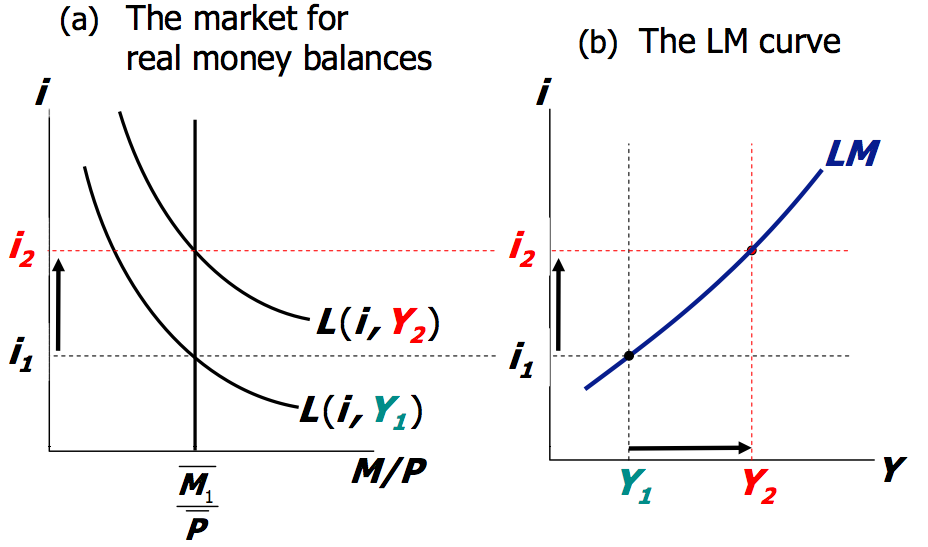
\includegraphics[height=3in]{images/LM-curve.png}
	\caption{LM-curve}
	\label{fig:images_LM-curve}
\end{figure}


\subsection{Aggregate expenditure, the interest rate and the exchange rate: the IS curve} % (fold)
\label{sub:aggregate_expenditure_the_interest_rate_and_the_exchange_rate_the_is_curve}
Consumptio function	
\begin{equation}
	C(Y, Y_+^e) =c_1Y+c_2Y_+^e
\end{equation}
can be simplified to $C(Y)$

Investment function
\begin{equation}
	I(i, Y_+^e) = b_1Y_+^e+b_2i
\end{equation}
can be simplified to $I(i)$


Real exchange rate
\begin{equation}
	\label{eq:real_exc_rate}
	R = E \frac{P^{\text{world}}}{P}
\end{equation}

import function
\begin{equation}
	IM = m_1Y-m_2R
\end{equation}

export function
\begin{equation}
	EX=x_1Y^{\text{world}}+x_2R
\end{equation}
Putting the last 4 equations into $Y = C + I + G + NX$ yields
\begin{equation}
	i = -\frac{1-c-m_1}{b}Y+\frac{x_2+m_2}{b}R+\frac{\overline I+G+x_1Y^{\text{world}}}{b}
\end{equation}

\begin{figure}[htbp]
	\centering
		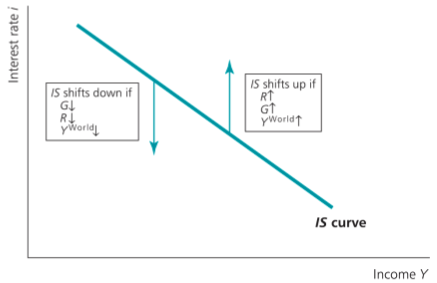
\includegraphics[height=3in]{images/IS-curve.png}
	\caption{$IS$-curve}
	\label{fig:images_LM-curve}
\end{figure}

\textbf{The $LM$-curve is for the money market (money supply $M$)\\and\\the $IS$-curve is for the goods market $I$, $C$ and $NX$}

% paragraph short_run_equilibrium (end)

% subsection aggregate_expenditure_the_interest_rate_and_the_exchange_rate_the_is_curve (end)

% section money_interest_rates_and_the_global_economy (end)


\section{Exchange rates and the balance of payments} % (fold)
\label{sec:exchange_rates_and_the_balance_of_payments}
under flexible exchange rate $OR=0 \Rightarrow CA=-CP$

the current account is determined by
\begin{equation}
	CA \equiv NX = EX -IM =-m_1Y+ x_1Y^{\text{world}}+(x_2+m_2)R
\end{equation}

and the capital account by
\begin{equation}
	CP = \kappa(i-i^{\text{world}})
\end{equation}
putting the last 3 equations together yields
\begin{equation}
	 i=i^{\text{world}}+\frac{m_1}{\kappa}Y-\frac{x_1}{\kappa}Y^{\text{world}}-\frac{m_2+x_2}{\kappa}R
\end{equation}

The 3 endogenous variables of the IS-LM-FE (or Mundell-Fleming) model are $Y, i, R$. Note that $R=E$ when $P=P^{\text{world}}$ because of \ref{eq:real_exc_rate}.
% section exchange_rates_and_the_balance_of_payments (end)


\section{Macroeconomic Accounting}

\begin{equation}
	BP = CA + CP + OR = 0
\end{equation}
Simplification
\begin{itemize}
	\item $OR=0$: exchange rates flexible
	\item $CA=NX$, if capital immobility: $NX=0$
\end{itemize}


\section{IS-LM-FE Modell - Mundell Fleming Model}
LM-curve is (at equilibrium $L=M=\overline M$)
\begin{equation}
	i = \frac{k}{h}Y-\frac{1}{h}\overline M
\end{equation}
IS-curve is ($Y = C+I+G+NX$ and solving for $i$)
\begin{equation}
	i = -\frac{1-c+m_1}{b}Y+ \frac{\overline I + G + x_1Y^{\text{world}}}{b}+\frac{x_2+m_2}{b}R
\end{equation}

The general FE-curve reads
\begin{equation}
	i = i^{\text{world}}+\frac{m_1}{\kappa}Y-\frac{x_1}{\kappa}Y^{\text{world}}-\frac{m_2+x_2}{\kappa}R
\end{equation}
most of the time we assume $\kappa\rightarrow\infty$ and thus
\begin{equation}
	i = i^{\text{world}}
\end{equation}

\paragraph{Multiplier} % (fold)
\label{par:multiplier}
is the partial derivative with respect to a certain parameter, for $G$ it is	
\begin{equation}
	\frac{\partial Y}{\partial G}
\end{equation}
% paragraph multiplier (end)

\subsubsection{Endogenous vs exogenous variables}
the endogenous variables are \textbf{either}:
\begin{itemize}
	\item $Y, i$ and $R$
	\item $Y$, $i$ and $M$
\end{itemize}
The exogenous variables are $G, i^{\text{world}}, Y^{\text{world}}$ and $M$ or $i$

\section{Aggregate Supply Curve}
\begin{equation}
	p = p^e+\lambda(Y-Y^*)
\end{equation}
where $p\equiv\ln{P}$ (percentage change rather than linear change)

\paragraph{Long-run $AS$ curve} % (fold)
\label{par:long_run_as_curve}
\begin{equation}
	Y = Y^*
\end{equation}
% paragraph long_run_as_curve (end)

\section{Aggregate Demand ($AD$ curve)}

\paragraph{$AD$ curve under flexible exchange rate} % (fold)
\label{par:_ad_curve_under_flexible_exchange_rate}
\begin{equation}
	P = a -bY +\text{other factors}[M(+),i^w(+),\epsilon^e(+)]
\end{equation}
and
\begin{equation}
	p = m-bY+h(i^w+\epsilon^e)
\end{equation}
% paragraph _ad_curve_under_flexible_exchange_rate (end)


\paragraph{$AD$ curve under flexible exchange rate} % (fold)
\label{par:_ad_curve_under_flexible_exchange_rate}
\begin{equation}
	P = a -bY +\text{other factors}[E(+),P^w(+),G(+),Y^w(+),i^w(-),\epsilon^e(-)]
\end{equation}
and
\begin{equation}
	p = e + p^w-bY+\gamma Y^w+\delta G-f(i^w+\epsilon^e)
\end{equation}
% paragraph _ad_curve_under_flexible_exchange_rate (end)

\section{$SAS$-curve}
\begin{equation}
	\pi = \pi^e +\lambda(Y-Y^*) = p-p_{-1}
\end{equation}
\section{$DAD$-curve}
\paragraph{$DAD$-curve under flexible exchange rate} % (fold)
\label{par:_dad_curve_under_flexible_exchange_rate}

% paragraph _dad_curve_under_flexible_exchange_rate (end)
\begin{equation}
	\pi = \mu-bY+bY_{-1}+h(\Delta i^w+\Delta \epsilon^e)
\end{equation}
where $\pi = p-p_{-1}$ and $\mu=m-m_{-1}$
\end{document}